
Experiments measuring the error after moving the camera in specific increments using the FVR based methods and other methods from the literature are presented in this section. For these experiments, one camera frame of an indoor environment was captured using the Asus Xtion Pro Live active camera. The camera was then moved (translated) by different amounts, 5 cm, 10 cm and 15 cm. The 2D and 3D Feature matching RANSAC methods (FM2D, FM3D), ICP and PCA methods were all tested. The results for the FVR, FFVR and FVR-3D methods are also presented. FM3D, FVR and FVR-3D require the 3D frames be quantized into $256\times 256\times 256$ volumes. \\

Different levels of noise were added to both frames prior to 3D registration to measure each method's ability to register frames with large amounts of noise. The Signal to Noise Ratio (SNR) metric is used to describe the noise added to both captured frames, prior to any registration. This noise effects any registration method's ability to accurately estimate the transformation separating two sets of data. In a given experiment, a noise range value of $x$ means random noise was added in the range [$\frac{-x}{2}$, $\frac{x}{2}$] to a signal within the range [0, 1]. Reconstruction error is measured in mean squared error (as presented in section \ref{metricsSection}). \\

Table \ref{table:trans} shows the results of these tests which, illustrate the FVR's robustness to noise whilst registering frames which are captured during different camera translation intervals. Each sub-table is labelled with a distance in centimetres in which frames were separated prior to registration. The first two columns represent the amount of noise added both in terms of noise-range and the subsequent Signal to Noise ratio computed from it. The remaining columns represent the registration error using the Mean Squared Error metric. Errors above 30 are capped, the final row of each table shows the average error for every noise level. \\

%translation
\begin{table}[!htb]
\centering
\caption{Translation Tracking}
\scalebox{1.0}{
\begin{tabular}{ccccccccc}
\\ \textbf{5cm} &   &   &   &   &   &   &   &   \\ 
Noise & SNR & \textbf{FM2D} & \textbf{FM3D} & \textbf{ICP} & \textbf{PCA} & \textbf{FVR} & \textbf{FFVR} & \textbf{FVR-3D} \\ \hline
0 & $\infty$ & 5.07 & 4.75 & 12.35 & 3.73 & 4.04 & 30 & 6.24 \\
0.1 & 20db & 18.96 & 30 & 30 & 2.33 & 2.73 & 14.6 & 5.63 \\
0.25 & 12db & 5.12 & 4.3 & 2.03 & 4.2 & 4.13 & 5.51 & 2.3 \\
0.5 & 6db & 5.61 & 1.95 & 3.71 & 6.83 & 3.7 & 7.73 & 2.83 \\
0.75 & 2.5db & 5.02 & 8.57 & 6.41 & 20.94 & 2.24 & 6.5 & 4.33 \\
Average & - & 7.96 & 9.91 & 10.91 & 7.61 & 3.37 & 12.87 & 4.27 \\
\\ \textbf{10cm} &   &   &   &   &   &   &   &   \\ 
Noise & SNR & \textbf{FM2D} & \textbf{FM3D} & \textbf{ICP} & \textbf{PCA} & \textbf{FVR} & \textbf{FFVR} & \textbf{FVR-3D} \\ \hline
0 & $\infty$ & 15.35 & 30 & 10.26 & 16.87 & 3.47 & 30 & 7.07 \\
0.1 & 20db & 18.2 & 15.36 & 6.24 & 30 & 3.89 & 30 & 11.45 \\
0.25 & 12db & 30 & 24.12 & 6.02 & 20.12 & 5.4 & 30 & 7.53 \\
0.5 & 6db & 30 & 4.42 & 5 & 3.96 & 4.65 & 30 & 9.47 \\
0.7 & 2.5db & 7.27 & 8.57 & 3.98 & 7.85 & 15.45 & 30 & 4.3 \\
Average & - & 20.16 & 16.49 & 6.3 & 15.76 & 6.57 & 30 & 7.96 \\
\\ \textbf{15cm} &   &   &   &   &   &   &   &   \\ 
Noise & SNR & \textbf{FM2D} & \textbf{FM3D} & \textbf{ICP} & \textbf{PCA} & \textbf{FVR} & \textbf{FFVR} & \textbf{FVR-3D} \\ \hline
0 & $\infty$ & 30 & 30 & 7.85 & 30 & 25.87 & 30 & 30 \\
0.1 & 20db & 30 & 30 & 7.13 & 30 & 12.27 & 30 & 30 \\
0.25 & 12db & 15.17 & 30 & 30 & 30 & 8.1 & 12.52 & 30 \\
0.5 & 6db & 30 & 30 & 11.11 & 30 & 10.13 & 11.09 & 30 \\
0.7 & 2.5db & 30 & 30 & 10.31 & 20.59 & 7.79 & 30 & 30 \\
Average & - & 27.03 & 30 & 13.28 & 28.12 & 12.83 & 22.44 & 30 \\
\\
\end{tabular}}
\\
\label{table:trans}
\end{table}


Results show that the basic FVR method is generally the most accurate in terms of registration across the range of camera translation magnitudes and noise levels. In comparison, the FFVR method reduces processing time at the expense of accuracy and robustness over a wide-baseline. Results generally show that FFVR is only capable of up to 5 cm of translation registration. FVR-3D and the 2D Feature Matching method can register 5-10 cm with larger levels of noise. However, both methods fail to register the full 15cm of camera translation well. In both the 5cm and the 15cm experiments, the FVR method has the lowest average error, and the second lowest in the 10cm camera translation tests. \\

ICP performed next best, capable of performing well up to 15cm of translation, but failing to register twice during the tests. PCA could handle up to 10 cm of translation but often had larger registration errors. For the 15 cm translation tests, the FVR performed the best followed by ICP, which failed once but outperformed FVR within the two lowest noise brackets. \\


It can be shown that, despite being limited to a single axis of rotation, the FVR algorithm can consistently register camera movements up to 15 cm better than other algorithms from the literature. To put these camera translations into perspective at video frame rates, a displacement of 10 cm per frame equates to camera velocity of 3 m/s, this is twice the average person's walking speed making both the FVR method and FVR-3D suitable for many applications. \\


\subsection{Camera Rotation Tracking}
\label{Sec:CamRoteTrackExp}

Table \ref{table:rote} shows the results for camera rotation experiments. These experiments were captured with the Asus Xtion Pro Live camera using the same scene as in section \ref{Sec:CamTransTrackExp}. 3D frames of these scenes are separated by 10, 20 and 30 degrees of camera rotation about the y-axis. These degrees were chosen because they are significantly large enough to be difficult for these algorithms to register against. Again, different levels of noise were added to each frame prior to registration. This experiment was designed to test the robustness of the FVR based methods in registering camera pose. \\


%rotation
\begin{table}[!htb]
\centering
\caption{Rotation Tracking}
\scalebox{1.0}{
\begin{tabular}{ccccccccc}
\\ \textbf{10deg} &   &   &   &   &   &   &   &   \\ 
Noise & SNR & \textbf{FM2D} & \textbf{FM3D} & \textbf{ICP} & \textbf{PCA} & \textbf{FVR} & \textbf{FFVR} & \textbf{FVR-3D} \\ \hline
0 & $\infty$ & 0.17 & 9.77 & 0.19 & 0.3 & 0.18 & 0.35 & 4.05 \\
0.1 & 20db & 0.21 & 0.41 & 0.17 & 0.67 & 0.15 & 0.21 & 10.54 \\
0.25 & 12 & 0.16 & 0.34 & 0.13 & 0.39 & 0.15 & 0.44 & 5.44 \\
Average & - & 0.18 & 3.51 & 0.16 & 0.45 & 0.16 & 0.33 & 6.68 \\
\\ \textbf{20deg} &   &   &   &   &   &   &   &   \\ 
Noise & SNR & \textbf{FM2D} & \textbf{FM3D} & \textbf{ICP} & \textbf{PCA} & \textbf{FVR} & \textbf{FFVR} & \textbf{FVR-3D} \\ \hline
0 & $\infty$ & 1.37 & 13.1 & 1.81 & 30 & 7.29 & 1.32 & 3.18 \\
0.1 & 20db & 1.35 & 30 & 30 & 2.97 & 0.7 & 2.03 & 1.92 \\
0.25 & 12db & 1.6 & 3.26 & 30 & 0.64 & 1.54 & 4.29 & 2.24 \\
Average & - & 1.44 & 15.45 & 20.60 & 11.20 & 3.18 & 2.55 & 2.45 \\
\\ \textbf{30deg} &   &   &   &   &   &   &   &   \\ 
Noise & SNR & \textbf{FM2D} & \textbf{FM3D} & \textbf{ICP} & \textbf{PCA} & \textbf{FVR} & \textbf{FFVR} & \textbf{FVR-3D} \\ \hline
0 & $\infty$ & 3.87 & 10.15 & 3.16 & 9.97 & 2.11 & 5.68 & 3.63 \\
0.1 & 20db & 3.77 & 30 & 30 & 30 & 3.84 & 2.82 & 1.39 \\
0.25 & 12db & 3.68 & 2.76 & 5.12 & 5.78 & 3.3 & 7.15 & 6.38 \\
Average & - & 3.77 & 14.30 & 12.76 & 15.25 & 3.08 & 5.22 & 3.8 \\
\\
\end{tabular}}
\\
\label{table:rote}
\end{table}

In the first sub-table, registration errors for 10 degrees of rotation are presented. Results show that the FVR method outperforms the other methods. Here, ICP performs next best followed by the 2D Feature Matching method. This was expected as the FVR method was designed to be both robust to noise and to be able to handle larger rotations. In the 20 degree and 30 degree tests, the FVR method performs better than the other algorithms in terms of having lower registration error. FFVR and FVR-3D also worked well at different noise levels up to 30 degrees of rotation. FVR-3D was found to be as robust as ICP at registering rotation but not as accurate as the 2D Feature Matching method. In the 20 degree rotation experiments, the 2D feature matching method was shown to perform best in terms of average error, but in the 30 degree experiments, FVR was the top performer. Again, when processing low quality depth data such as those generated by an active camera, the FVR based methods have reduced performance compared to other algorithms compared to processing higher quality depth data. \\ 

It should be noted that twelve degrees of camera rotation per frame is almost a full rotation per second in video rates. This is so fast that most cameras would acquire too much motion blur for registration to be possible. Therefore, this test indicates the robustness of the FVR method in comparison with the other algorithms within the context of camera pose estimation. \\


\subsection{Reconstructed Scenes}
\label{Sec:FVRQual1Exp}

\begin{figure}[!htb] 
        \centering
        \begin{subfigure}[b]{3.0in}
                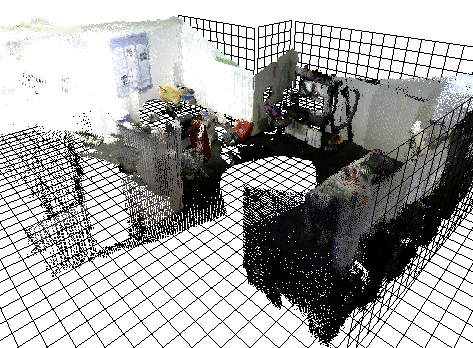
\includegraphics[width=3.0in]{images/ch2/unit21}
                \caption{Apartment}
                \label{fig:RECON_UNIT}
        \end{subfigure}
        \begin{subfigure}[b]{3.0in}
                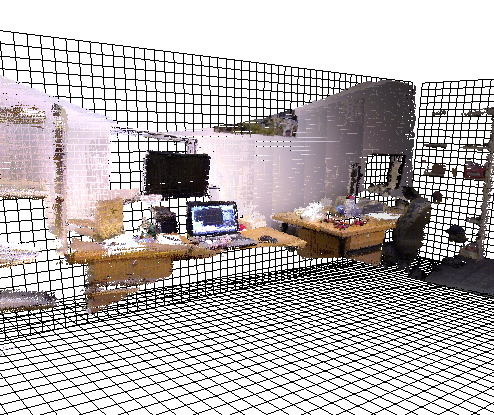
\includegraphics[width=3.0in]{images/ch2/officeA}
                \caption{Office}
                \label{fig:RECON_OFFICE}
        \end{subfigure}
        \begin{subfigure}[b]{3.0in}
                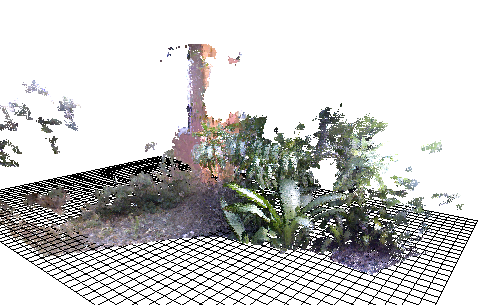
\includegraphics[width=3.0in]{images/ch2/outdoorA}
                \caption{Garden}
                \label{fig:RECON_GARDEN}
        \end{subfigure}
       \caption{Reconstructed Scenes.}
       \label{fig:RECONSTRUCTIONS}
\end{figure}

To assess qualitative reconstructions, three scenes were captured and registered using the FVR method. These scenes are the apartment scene, office scene and the garden scene. All three scenes were captured using the Asus Xtion Pro live active camera at 30 frames per second. For each scene, only one in every 30 frames was registered, constituting real time FVR performance. The apartment scene was generated by moving and rotating the camera around an apartment living room before moving towards the kitchen area. This scene contains an abundance of features and would be considered a basic test for most 3D reconstruction algorithms. The second scene is the office scene. This scene was generated by rotating the camera whilst zooming in and out on different objects within the room. Again, this scene was reconstructed by registering every 30th frame. Despite both scenes being trivial to reconstruct, most algorithms (especially feature matching based methods) would find registering large rotations (such as those present in this data) difficult. The garden scene is a difficult scene to reconstruct regardless of the reconstruction algorithm or technique used for registration. This scene was captured by rotating the camera around a garden outside the university. The scene contains many textures which are similar at the local level but are located in totally different locations. Therefore, the scene is difficult to reconstruct using local and feature based methods such as Feature Matching + RANSAC and ICP. \\


Reconstructions for the two indoor environments (apartment and office) as well as one outdoor environment (garden) are shown in Figures \ref{fig:RECON_UNIT}, \ref{fig:RECON_OFFICE} and \ref{fig:RECON_GARDEN}, respectively. \\

The apartment reconstruction was recorded by moving the Asus Xtion Pro Live active camera through a room and rotating the camera. Each frame was registered using the FVR algorithm. Some of the frames in the apartment scene contain walls which have few features. Between frames, walls also had colour contrast shifts. These shifts are due to the Asus camera's automatic contrast feature which adjusts contrast based on colour histograms. Despite these setbacks, accurate 3D reconstruction was achieved by the FVR method as illustrated in Figure \ref{fig:RECON_UNIT}. \\


The office reconstruction was also generated by rotating the Asus Xtion Pro Live active camera about the y-axis while moving the camera around the room. During rotation, the camera was focused on both foreground and background objects. Here, the entire video sequence was accurately registered. Despite the foreground and background focus, the global reconstruction is accurate. This scene, as in the apartment scene has usable texture which should not cause large amounts of texture confusion. These qualitative experiments show that despite being a closed form solution, the FVR has reconstruction accuracy comparable to existing feature based SLAM methods. \\


Typical feature based methods work well with indoor environments where local features are readily distinguishable and easy to match. They do not tend to work as well in complex outdoor scenes where feature confusion is likely. To assess performance in such outdoor scenes, a garden scene containing bushes, plants and a ground covering of bark and rocks was captured for testing. Again, this scene was captured using the Asus Xtion Pro Live active camera moving around the outdoor garden. The proposed FVR method produced a good quality reconstruction of this garden scene, as shown in Figure \ref{fig:RECON_GARDEN}. This shows that reconstruction approaches which integrate or make use of the FVR registration method may have an advantage in performing 3D reconstructions in these types of scenes, which commonly disturb many existing feature matching methods, as expressed in the literature.   

Reconstructions of the Parks, Plants and Table data set using the FVR, ICP and FM2D methods are shown in Figure \ref{fig:QualReconstructions2}. It can be seen that the FVR method could reconstruct the scene accurately. FM2D and ICP failed to generate a suitable reconstruction for this data set. This is likely due to the level of texture confusion present in the scene. The FVR based methods are more robust to texture confusion, since they make use of all of the data independent of salient points within the scene.


\begin{figure}[!htb] 
        \centering
        \begin{subfigure}[b]{3.0in}
                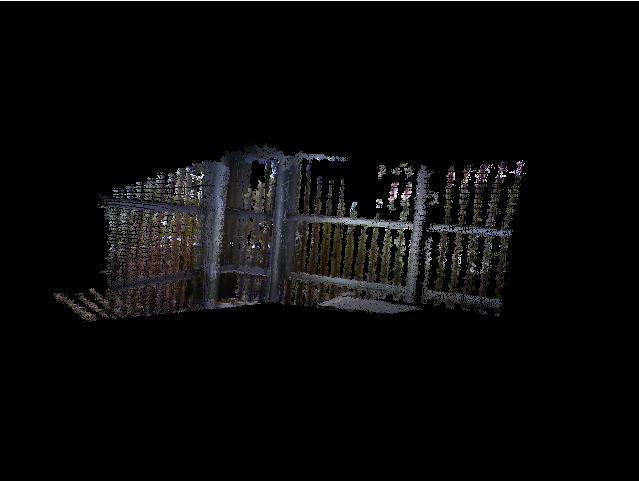
\includegraphics[width=3.0in]{images/results/qualitative_fvr_sota/plants_outdoors_FVR}
                \caption{FVR}
                \label{fig:qualrecon2FVR}
        \end{subfigure}
        \begin{subfigure}[b]{3.0in}
                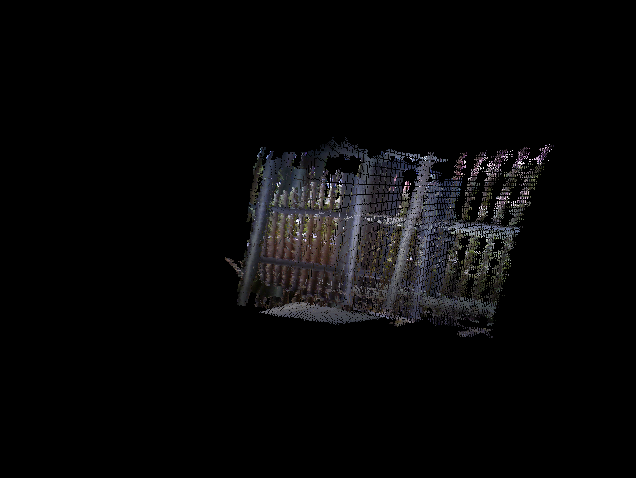
\includegraphics[width=3.0in]{images/results/qualitative_fvr_sota/plants_outdoors_ICP}
                \caption{ICP}
                \label{fig:qualrecon2ICP}
        \end{subfigure}
        \begin{subfigure}[b]{3.0in}
                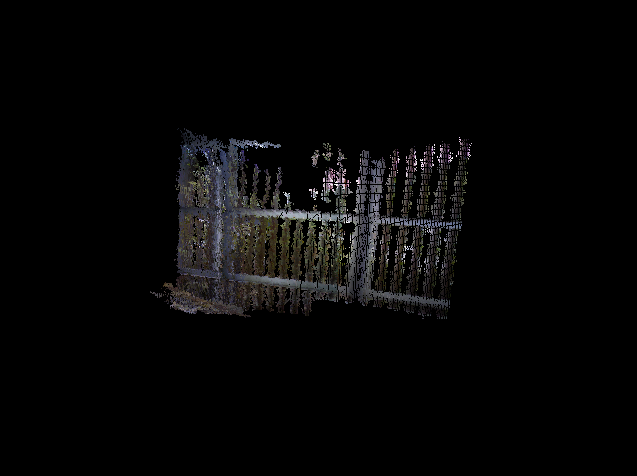
\includegraphics[width=3.0in]{images/results/qualitative_fvr_sota/plants_outdoors_FM2D}
                \caption{FM2D}
                \label{fig:qualrecon2FM2D}
        \end{subfigure}
       \caption{Reconstructions of the Parks, Plants and Table Scene Using FVR, ICP and FM2D.}
       \label{fig:QualReconstructions2}
\end{figure}

